
\chapter{Results}

\label{ch:results}

As a first step, I have conducted FEM micromagnetic simulations of single grains of greigite. The simulations were performed with the free software package \textit{micromag} by \citet{micromag}. Micromag is written in Python and C++ and extensively uses the free software collection of packages for automated solutions of partial differential equations by the FEM \textit{FEniCS} \citep{Fenics}. It uses a combination of energy minimisation (as an initial guess) and numerical solution of the LLGE. The demagnetising field is calculated with a transformation method as proposed by \citet{Brunotte} and similar to the implementation of \citet{Abert} with the exception of using spherical outer shells for treating the open boundary conditions insted of cuboids.\par

I have compared domain structures and hysteresis loops of octahedral grains of greigite with truncated octahedral grains (octahedra with chopped vertices). These are typical morphologies for greigite. Since the parameters of highly pure greigite were only recently measured by \citet{Chang} there aren't, as far as I know, micromagnetic FEM models of greigite. It is important to mention that these simulations do not consider thermal fluctuations so, technically they represent the behaviour of the material at 0 K though they are indicative of possible behaviour at finite but low temperatures.\par

I have created the geometries with the commercial software Maya (by Autodesk) and meshing with the commercial preprocessing software Trelis (by Csimsoft). Visualization of the results was done with the free sofware package Paraview. Figures (\ref{Fig2}) and (\ref{Fig3}) are meshes of an octahedral and a truncated octahedral grain. Note the spherical shells surrounding the material used for calculating the demagnetising field are meshed in a more coarse manner as there is no need for the elements outside the material to be smaller than the exchange length. The length of the sides of the tetrahedral elements in the material are {\raise.17ex\hbox{$\scriptstyle\sim$}}6 nm (exchange length for greigite is {\raise.17ex\hbox{$\scriptstyle\sim$}}7.5 nm).
\begin{figure}[ht]
\centering
\includegraphics[width=\columnwidth]{s_octa_g_mesh.eps}
\caption{Mesh of a 200nm octahedral grain.}
\label{Fig2}
\end{figure}
\begin{figure}[ht]
\centering
\includegraphics[width=\columnwidth]{c_octa_g_mesh.eps}
\caption{Mesh of a 200nm truncated octahedral grain.}
\label{Fig3}
\end{figure}

Figure (\ref{Fig4}) is possibly the most interesting solution so far. It shows the domain structure of an octahedral grain 200 nm across (side length {\raise.17ex\hbox{$\scriptstyle\sim$}}141 nm). At first glance the solution seems to be a vortex state, which would be expected from the size of the grain if we compare with a cube of the same side length. Actually, the vortex does not penetrate wholly the grain. There are two vortices formed superficially and their direction of rotation is opposite. Thus, inside the grain there is a core that holds a very uniform magnetisation along the direction of the easy axis. Figure (\ref{Fig5}) shows the magnetic flux from where it is seen that the directions of the vortices are opposite and the magnetisation is uniform inside the grain. We compare this with a vortex state obtained for a cube with side length {\raise.17ex\hbox{$\scriptstyle\sim$}}115 nm. I chose this size because then the octahedron and the cube have the same surface area to volume ratio. Figures (\ref{Fig6}) and (\ref{Fig7}) show this vortex state magnetisation configuration and its magnetic flux. Clearly this is a true vortex state. So, it seems that octahedral grains can remain in an almost SD state for bigger sizes than cubic shaped grains. This is even more clear in the simulation for the same 200 nm across octahedral grain but with its corners chopped. Figures (\ref{Fig8}) and (\ref{Fig9}) show that if the corners are chopped the superficial vortices are not formed and instead we have a simple flower state (a state that only deviates slightly from uniformity near the surfaces and corners).
\begin{figure}[ht]
\centering
\includegraphics[width=\columnwidth]{s_octa_g.eps}
\caption{Magnetisation of a 200nm octahedral grain.}
\label{Fig4}
\end{figure}
\begin{figure}[ht]
\centering
\includegraphics[width=\columnwidth]{s_octa_g_tube.eps}
\caption{Magnetic flux of a 200nm octahedral grain.}
\label{Fig5}
\end{figure}
\begin{figure}[ht]
\centering
\includegraphics[width=\columnwidth]{cube_octag.eps}
\caption{Magnetisation of a 115nm cubic grain. Vortex state.}
\label{Fig6}
\end{figure}
\begin{figure}[ht]
\centering
\includegraphics[width=\columnwidth]{cube_octag_tube.eps}
\caption{Magnetic flux of a 115nm cubic grain. Vortex state.}
\label{Fig7}
\end{figure}
\begin{figure}[ht]
\centering
\includegraphics[width=\columnwidth]{c_octa_g.eps}
\caption{Magnetisation of the 200nm octahedral grain with its corners chopped. Flower state.}
\label{Fig8}
\end{figure}
\begin{figure}[ht]
\centering
\includegraphics[width=\columnwidth]{c_octa_g_tube.eps}
\caption{Magnetic flux of the 200nm octahedral grain with its corners chopped. Flower state.}
\label{Fig9}
\end{figure}

To calculate hysteresis loops, first the material is driven to saturation with a high applied field. Once this state is achieved, the solution is taken as the initial condition of a following simulation with a smaller applied field. This is repeated until reaching zero applied field. Then, the field is augmented stepwise in the direction opposite to the initial field until reaching saturation. So far, I have only modelled hysteresis loops for smaller SD grains (both octahedrons and truncated octahedrons). Figures (\ref{Fig10}), (\ref{Fig11}) and (\ref{Fig12}) show hysteresis loops of a 60 nm across ({\raise.17ex\hbox{$\scriptstyle\sim$}}42 nm side length) octahedral grain of greigite with applied field along an easy axis ({111} crystallographic direction), a hard axis ({001}) and an axis lying between ({011}) respectively. For the same grain but with its corners chopped the same simulations were carried out and I found the coercivity of the truncated octahedrons to be {\raise.17ex\hbox{$\scriptstyle\sim$}}2$\times10^-6$ Tesla smaller. This was also observed for other sizes.
\begin{figure}[ht]
\centering
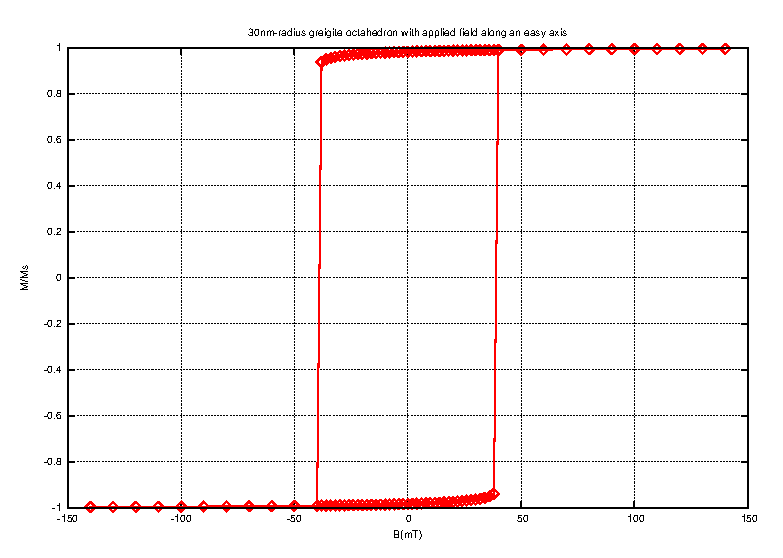
\includegraphics[width=\columnwidth]{B-M_30nm_looped_easy.eps}
\caption{Hysteresis loop of a 60nm across octahedral grain of greigite with applied field along an easy axis.}
\label{Fig10}
\end{figure}
\begin{figure}[ht]
\centering
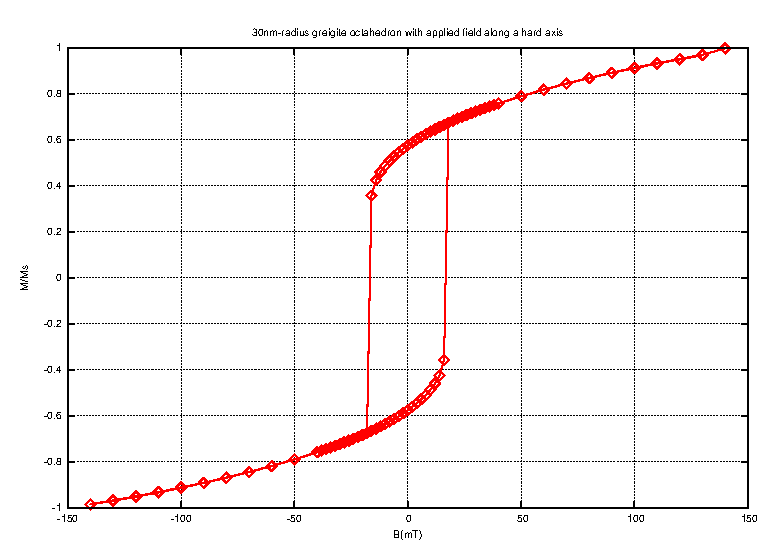
\includegraphics[width=\columnwidth]{B-M_30nm_looped_hard.eps}
\caption{Hysteresis loop of a 60nm across octahedral grain of greigite with applied field along a hard axis.}
\label{Fig11}
\end{figure}
\begin{figure}[ht]
\centering
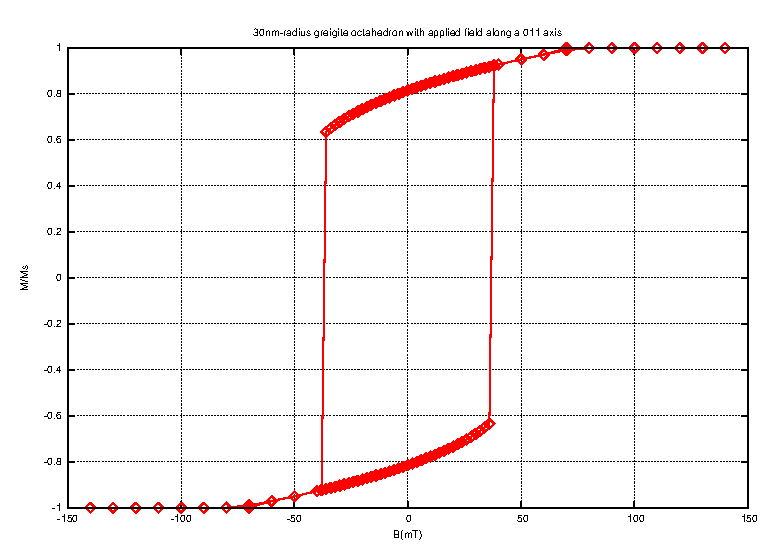
\includegraphics[width=\columnwidth]{B-M_30nm_looped_middle.eps}
\caption{Hysteresis loop of a 60nm across octahedral grain of greigite with applied field along a {011} axis.}
\label{Fig12}
\end{figure}